\section{Mise en place d'une connexion SSL/TLS mutualisée}

\subsection{Objectifs et pré-requis}

Nous cherchons ici à établir une connexion SSL/TLS mutualisée. \\

Pour cela, nous considérons sur le serveur possédant le serveur TLS que :
\begin{itemize}
    \item le serveur est une machine virtuelle hébergée dans le Cloud de Google ;
    \item l'OS utilisé est un Debian 64 ;
    \item le serveur Nginx est déjà installé \textbf{mais pas encore configuré} ;
    \item le nom de domaine utilisé est \textit{ultrae.eu} ;
    \item le site web est déjà créé dans \textit{/var/www/html/}.
\end{itemize}

\subsection{Paramétrage du serveur NGINX}

Pour pouvoir paramétrer nginx il faut :
\begin{enumerate}
    \item Générer à l'aide du pki (voir dev.pdf) :
    \begin{itemize}
        \item un certificat CA et sa clé privée ;
        \item un CSR signé par le CA.
    \end{itemize}
    \begin{figure}[h!]
	    \begin{center}
		    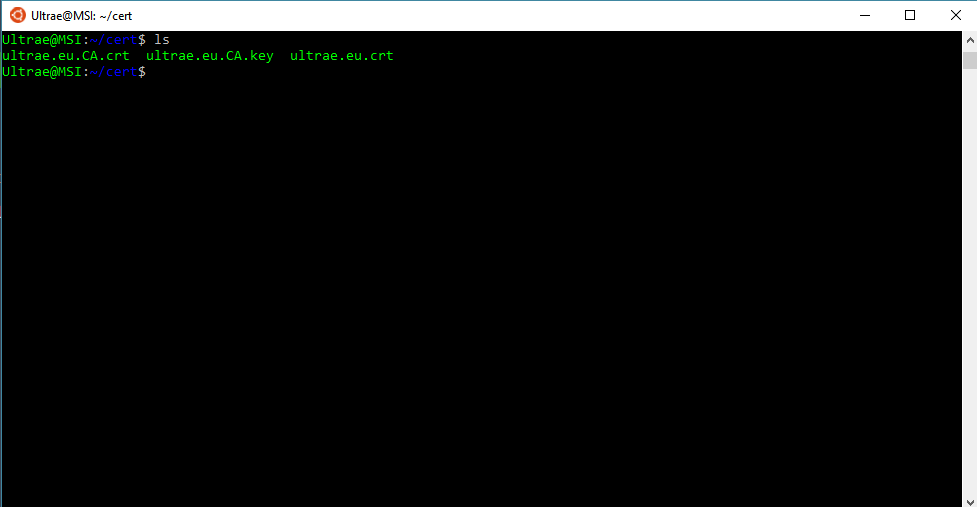
\includegraphics[scale=0.5]{Interception_Screenshots/mut01.png}
		    \caption{Affichage des certificats pour le TLS mutualisé}
	    \end{center}
    \end{figure}
    \FloatBarrier
    
    \item Les placer dans un dossier sur le serveur distant. 
    \begin{figure}[h!]
	    \begin{center}
		    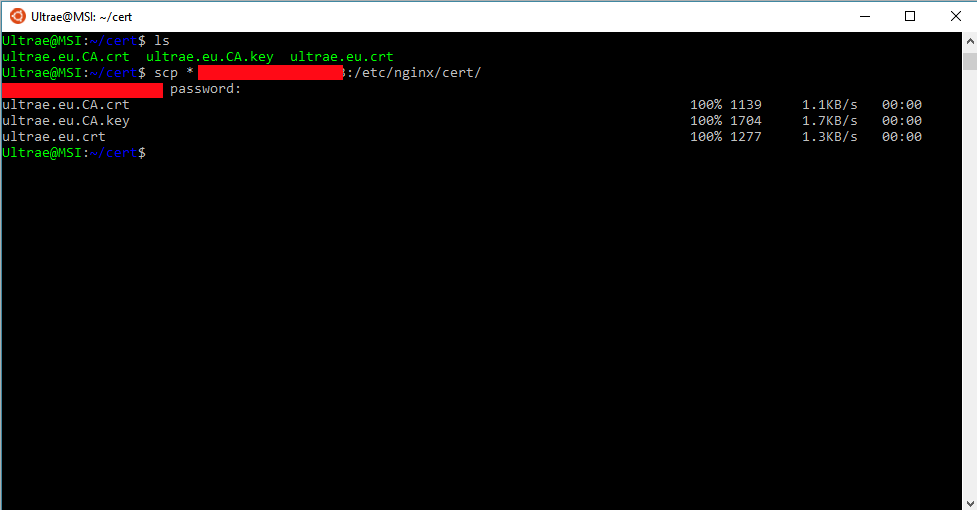
\includegraphics[scale=0.5]{Interception_Screenshots/mut02.png}
		    \caption{Mise en place des certificats pour le TLS mutualisé}
	    \end{center}
    \end{figure}
    \FloatBarrier
    
    \item Dans la configuration ssl de Nginx rajouter les lignes :
    \begin{itemize}
        \item \texttt{ssl\_certificate "/etc/nginx/cert/ultrae.eu.CA.crt";}
        \item \texttt{ssl\_certificate\_key "/etc/nginx/cert/ultrae.eu.CA.key";}
        \item \texttt{ssl\_client\_certificate "/etc/nginx/cert/ultrae.eu.crt";}
        \item \texttt{ssl\_verify\_client on.}
    \end{itemize}
    
    \item Ajouter dans le navigateur :
    \begin{itemize}
        \item le certificat du CA dans les certificats root trusted ;
        \item le certificat client dans les certificats personnels.
    \end{itemize}
\end{enumerate}

\subsection{Interception SSL/TLS sur une connexion TLS mutualisée}

Afin de pouvoir intercepter et pouvoir déchiffrer un flux chiffré entre un serveur TLS et un client s'authentifiant mutuellement, il faut :
\begin{itemize}
    \item Se connecter sur pfsense ;
    \item Dans \textbf{System -> Cert. Manager}, importer un CA ;
    \begin{figure}[h!]
	    \begin{center}
		    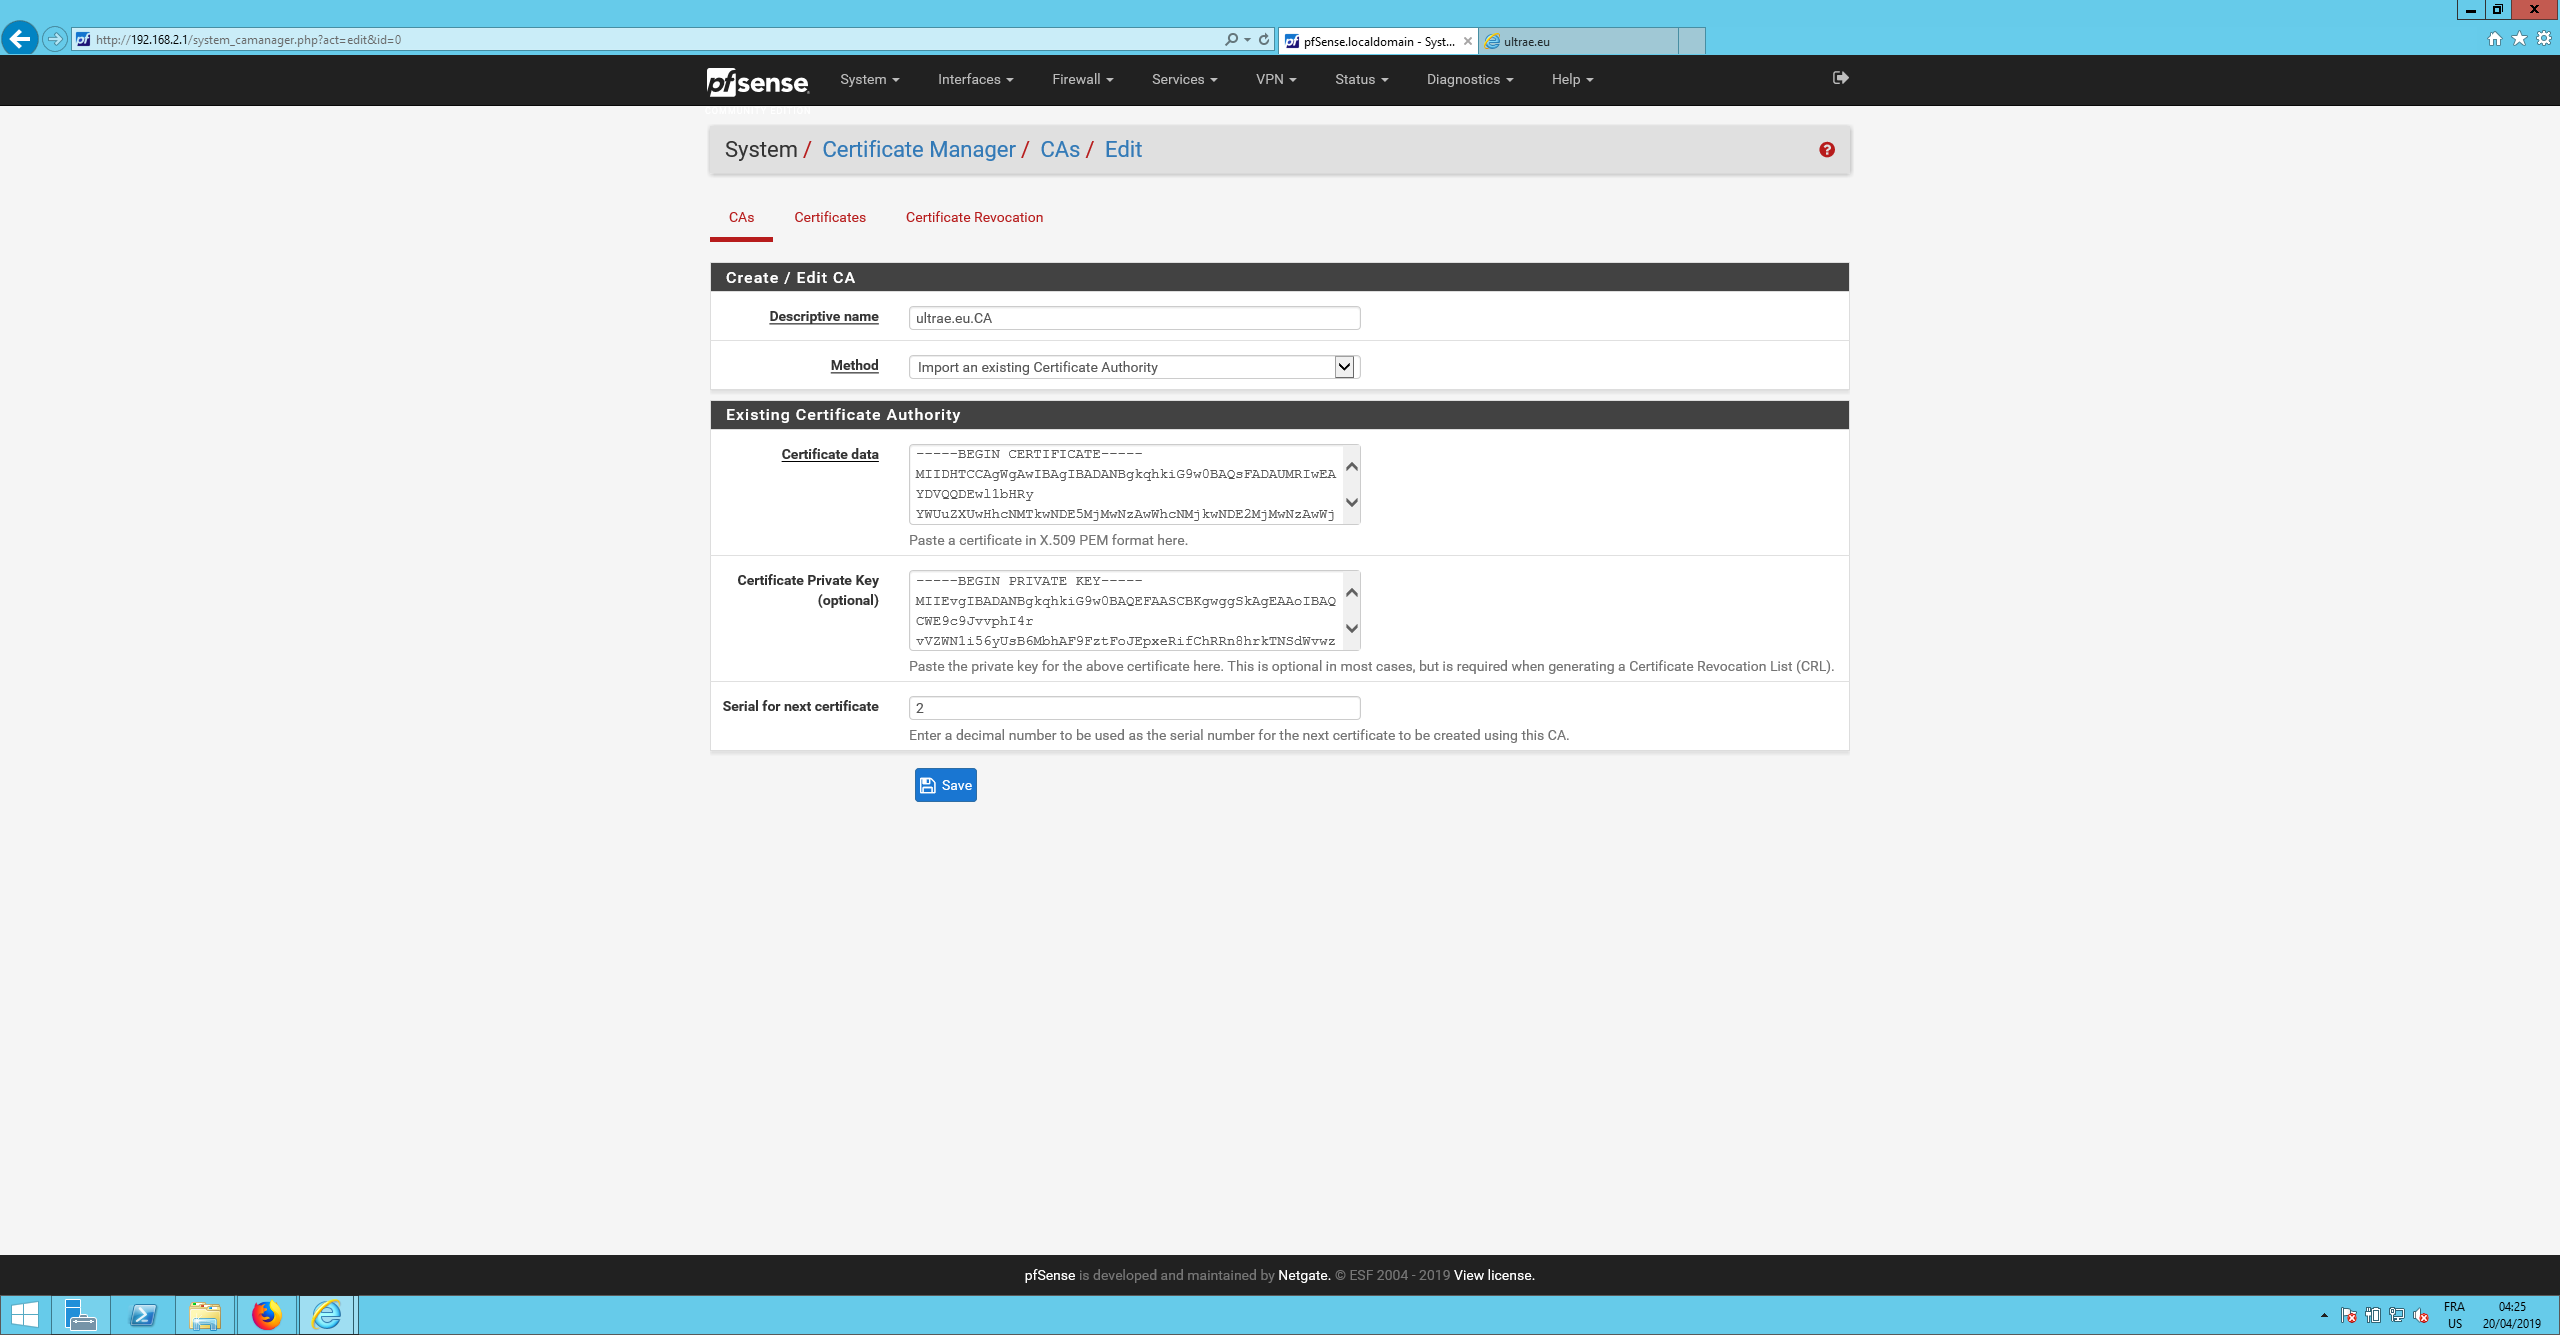
\includegraphics[scale=0.2]{Interception_Screenshots/mut03.png}
		    \caption{Importation du CA pour le TLS mutualisé}
	    \end{center}
    \end{figure}
    \FloatBarrier
    
    \item Dans l'onglet \textbf{Certificates}, importer un CSR ;
    \begin{figure}[h!]
	    \begin{center}
		    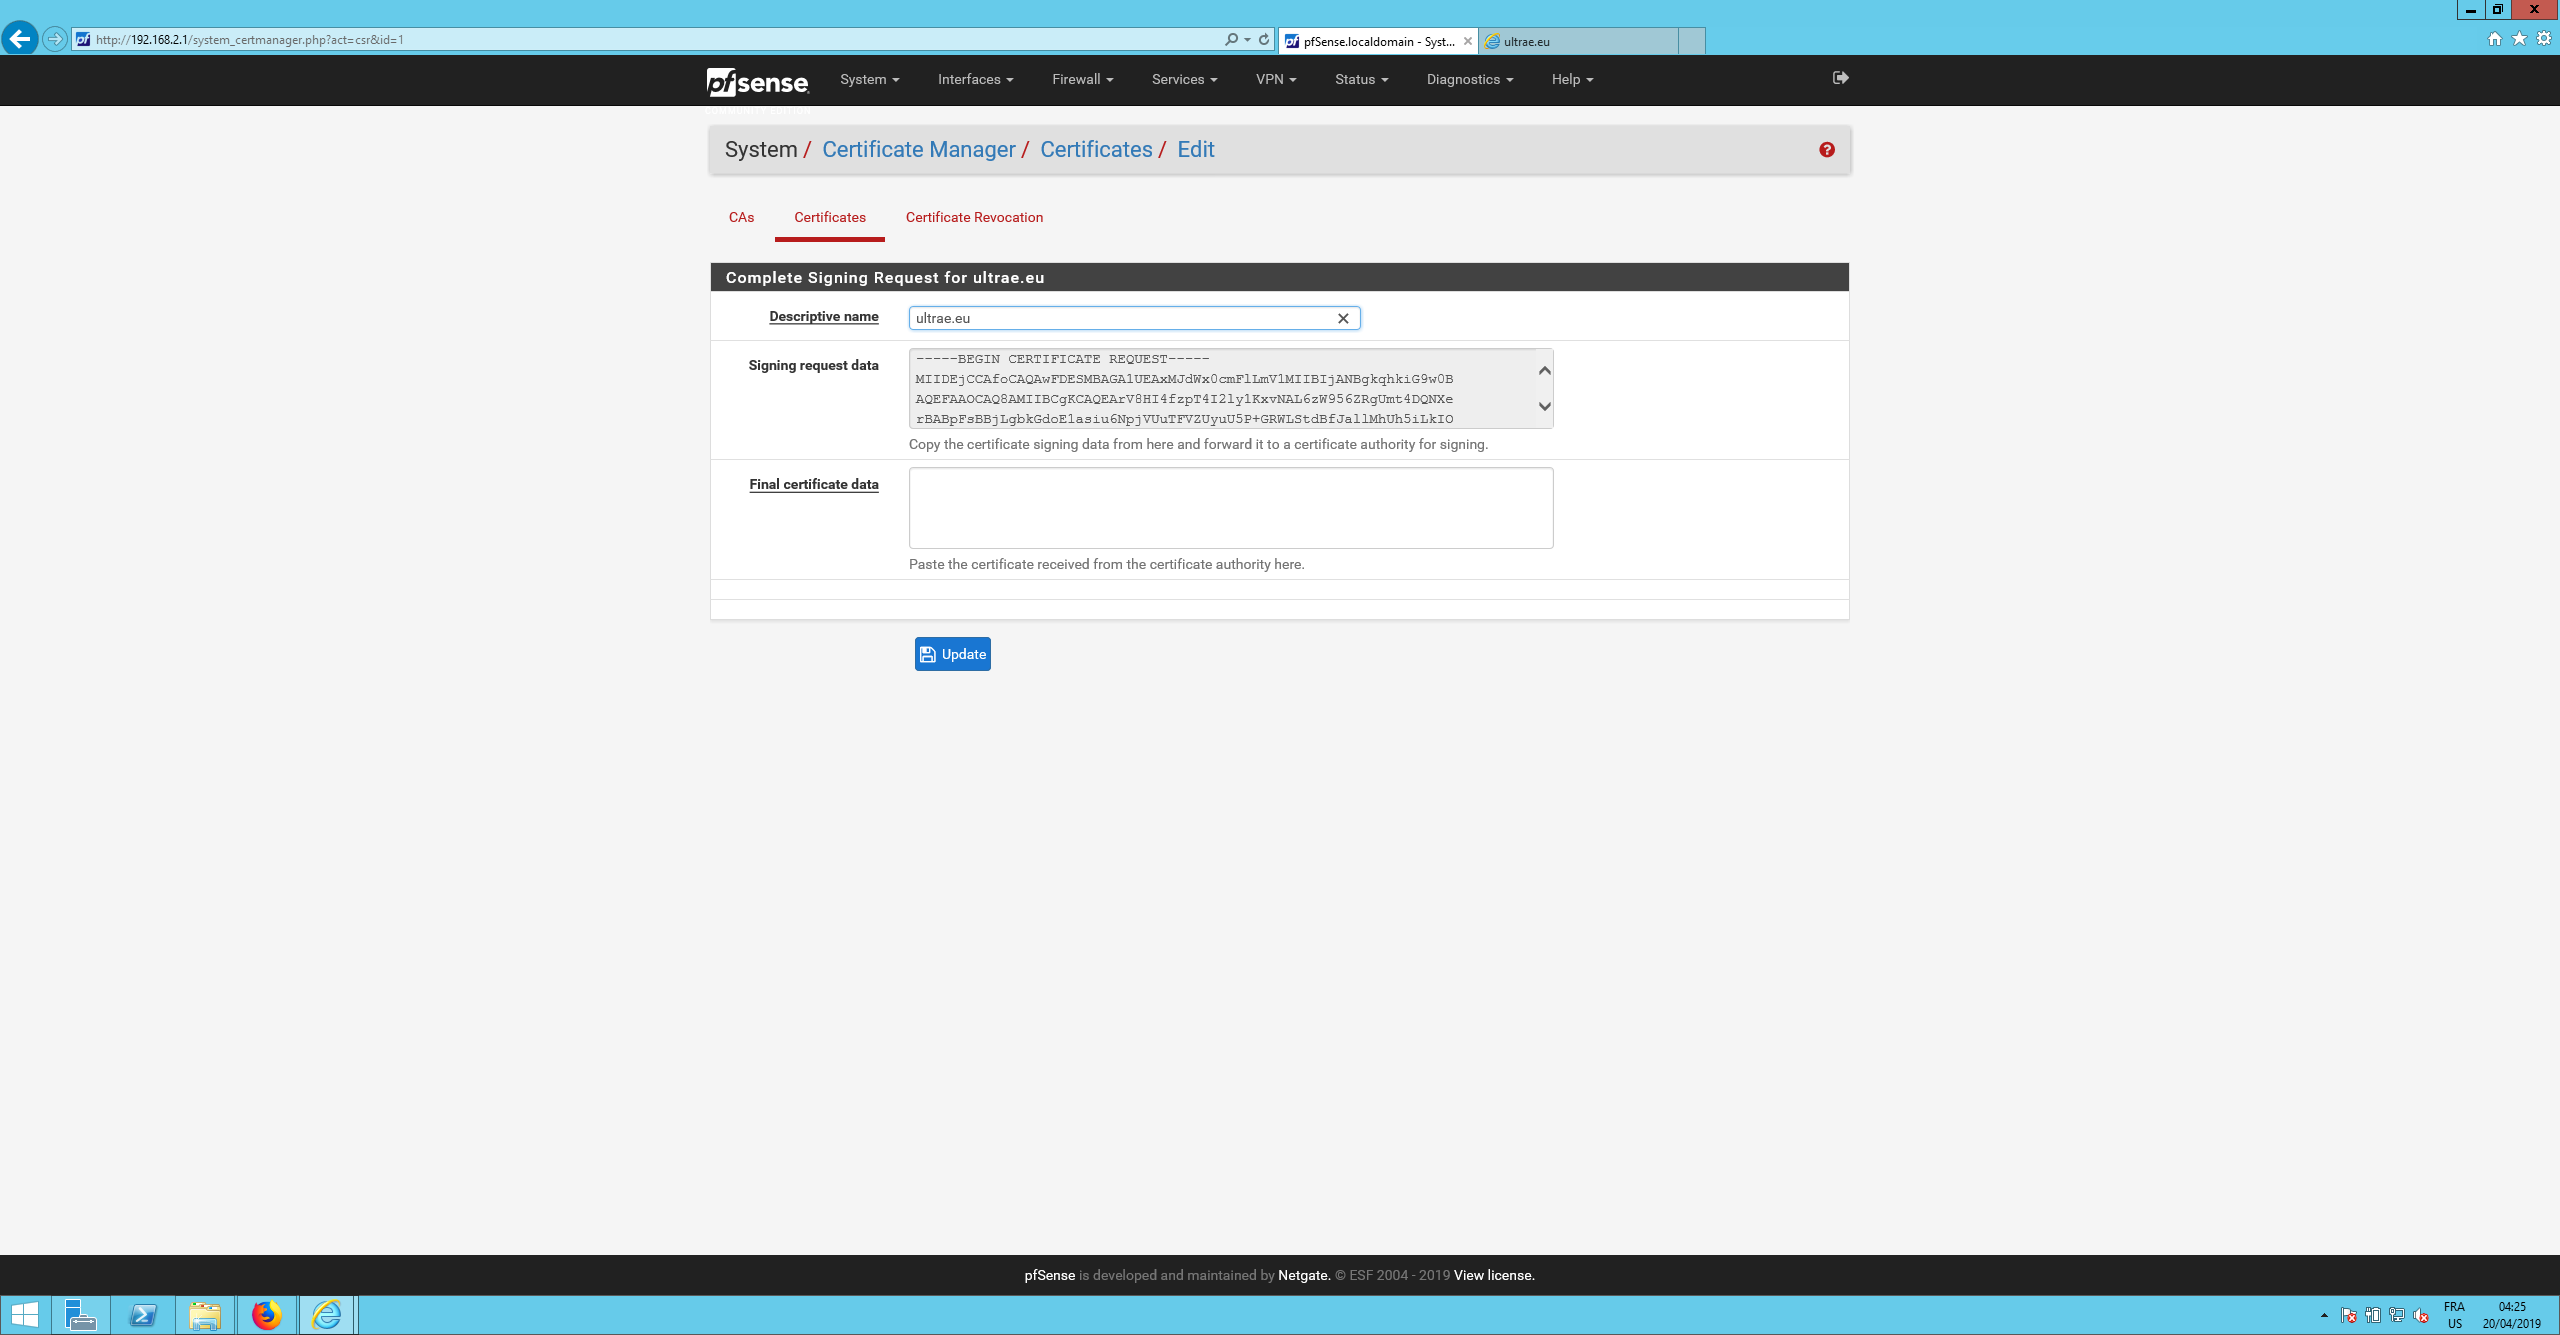
\includegraphics[scale=0.2]{Interception_Screenshots/mut04.png}
		    \caption{Importation du CSR pour le TLS mutualisé}
	    \end{center}
    \end{figure}
    \FloatBarrier
    
    \item Ajouter un nouveau certificat, selectionner la méthode \textit{Sign a Certificate Signing Request};
    \item Mettre \textit{ultrae.eu} dans \textit{Descriptive name} ;
    \item Mettre \textit{ultrae.eu.CA} dans \textit{CA to sign} ;
    \item Mettre \textit{sha512} dans \textit{Digest Algorithm} ;
    \item Mettre \textit{URI} et \textit{www.ultrae.eu} dans \textit{Alternative Names} ;
    \item Cliquer sur save.
    \begin{figure}[h!]
	    \begin{center}
		    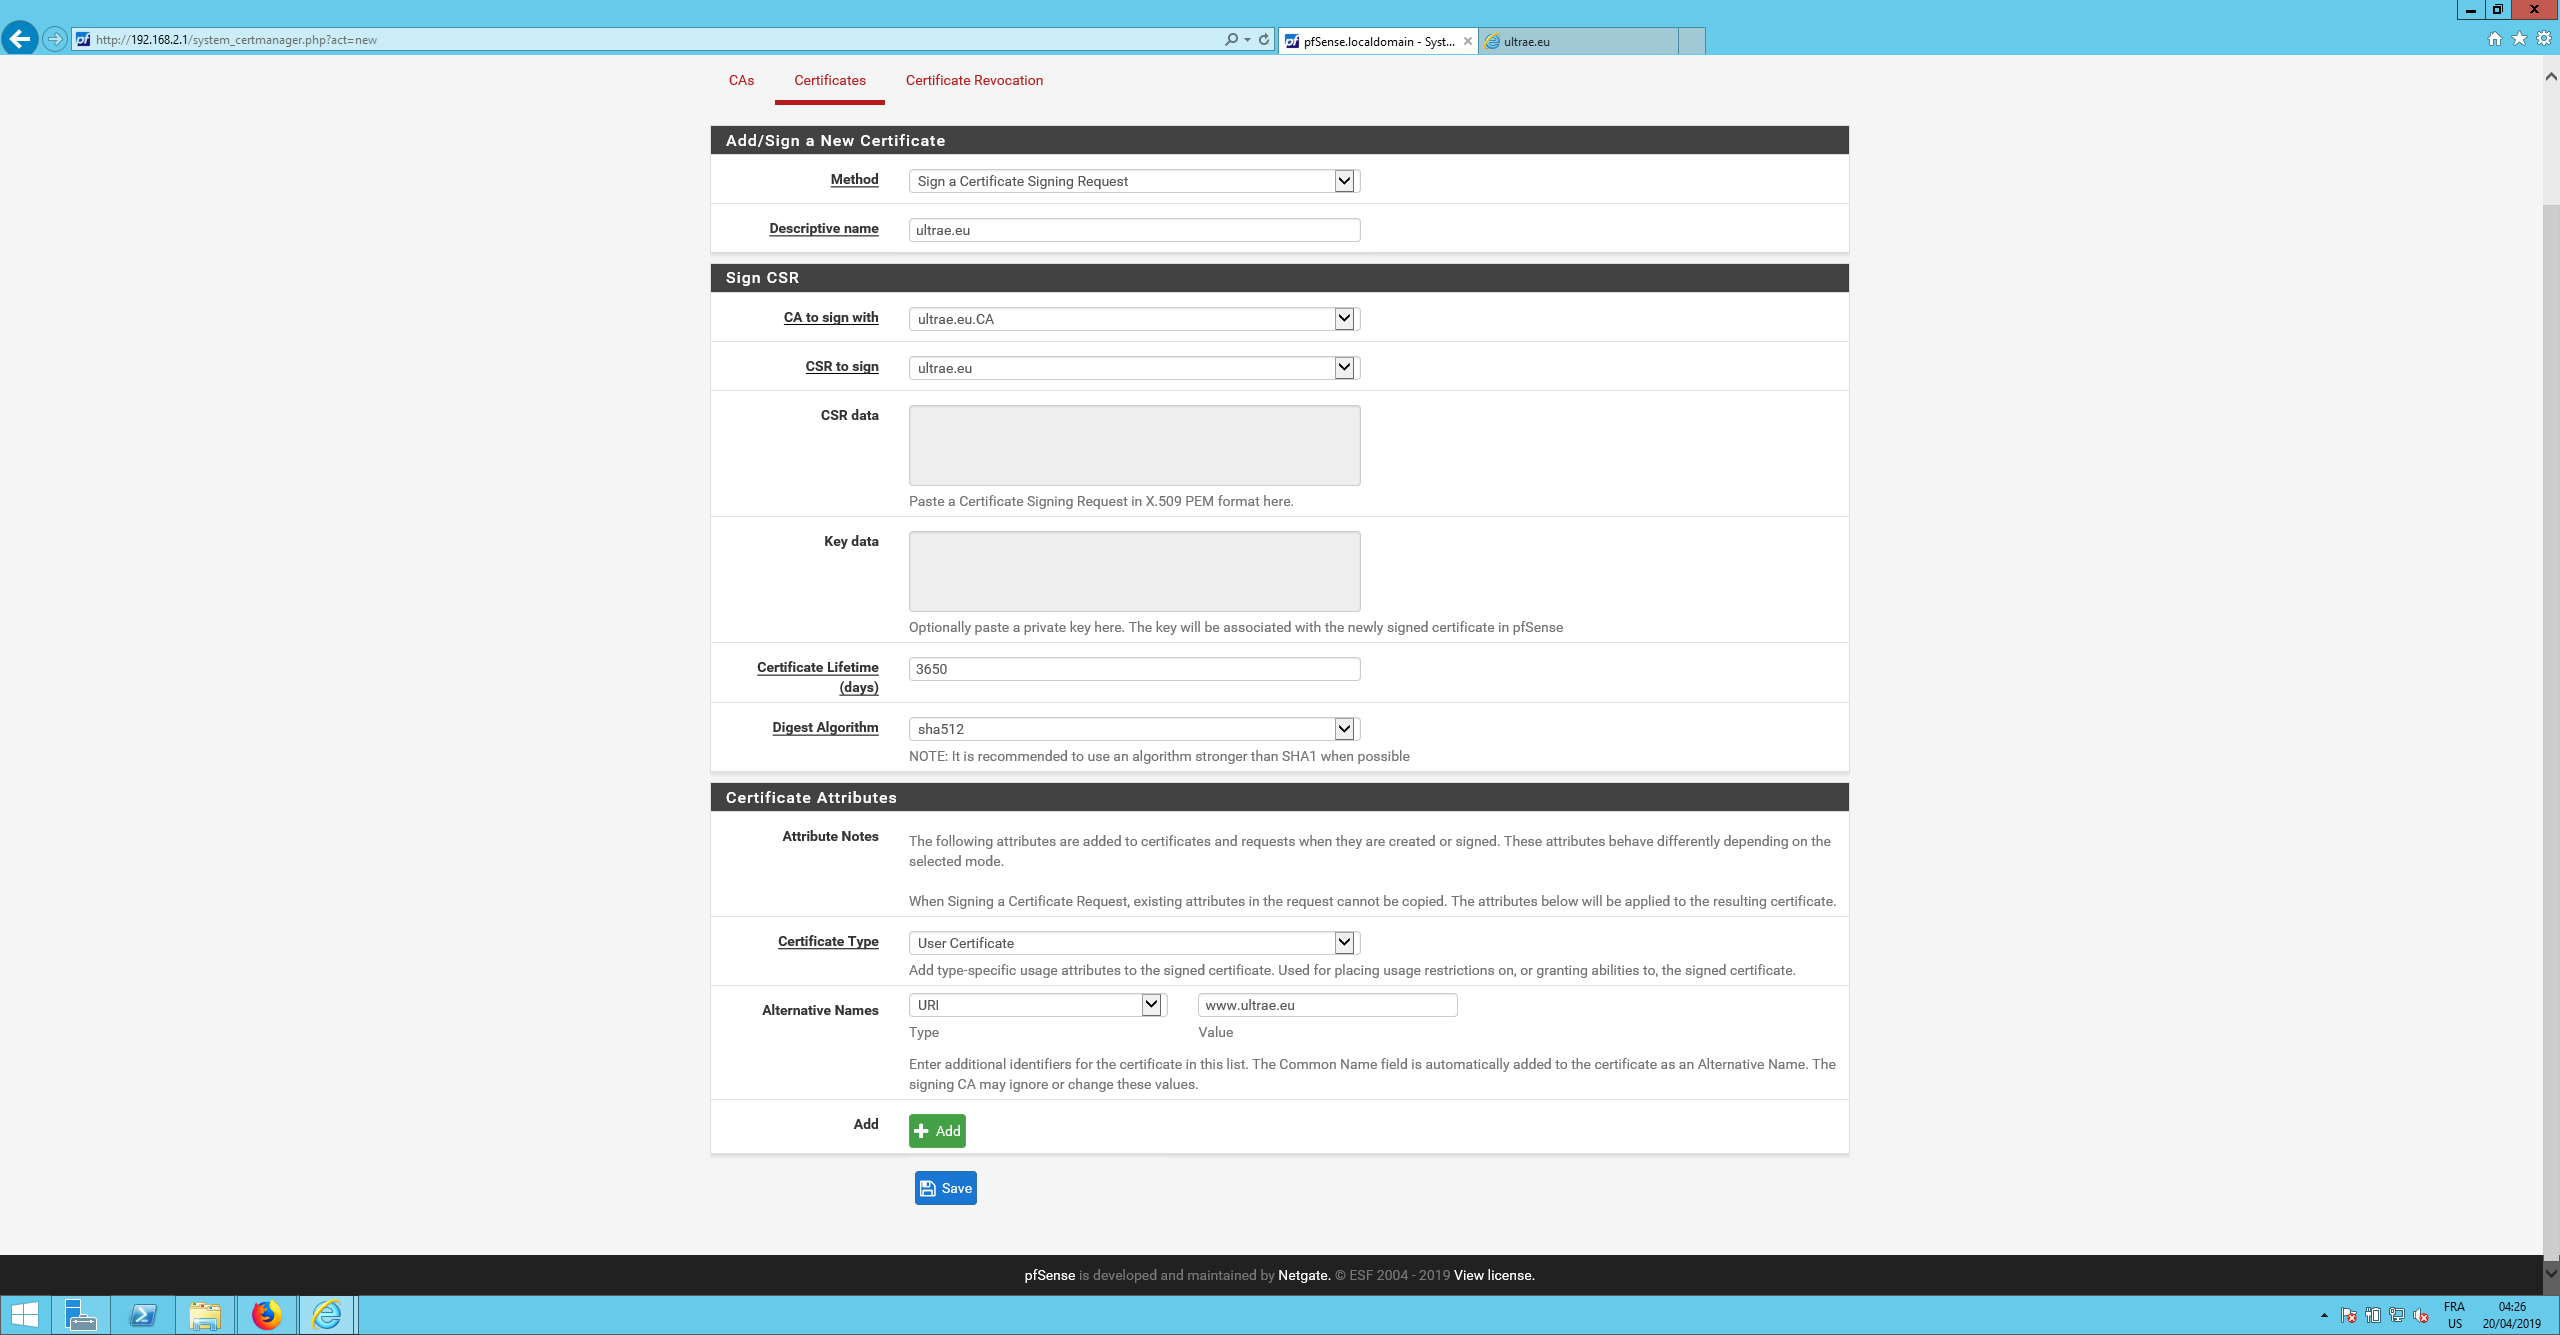
\includegraphics[scale=0.2]{Interception_Screenshots/mut05.png}
		    \caption{Signature du CSR pour le TLS mutualisé}
	    \end{center}
    \end{figure}
    \FloatBarrier
\end{itemize}
-